
\chapter{La célula solar\label{cha:Celula}}

\nocite{LopezAraujo1986}


\section{Teoría de Semiconductores}


\subsection{Modelo de bandas de energía}

Supongamos una red cristalina formada por átomos. Según los postulados
de la Mecánica Cuántica, los electrones de un átomo aislado pueden
existir únicamente en determinados estados de energía. A medida que
disminuye la distancia interatómica comienza a observarse la interacción
mutua entre los átomos hasta formarse un sistema electrónico único.
Las fuerzas de repulsión y atracción entre los átomos encontrarán
su equilibrio cuando los átomos estén separados por la distancia interatómica
típica del cristal que se trate. La separación real entre átomos en
el cristal será aquella para la cual la energía del sólido sea mínima.

En un sólido el número de átomos es tan elevado que los niveles de
energía forman bandas continuas de energía. Los electrones asociados
a los átomos del sólido llenan estas bandas en orden ascendente. La
banda de mayor energía completamente ocupada se denomina banda de
valencia (electrones ligados a átomos). La siguiente banda, parcialmente
ocupada o vacía, se denominada banda de conducción (electrones desligados
de átomos). Estas bandas pueden estar separadas por otra banda de
energías que corresponde a estados no permitidos, y de ahí que a esta
banda se la denomine banda prohibida, o bien pueden estar solapadas
permitiendo una transición fácil de una a otra. 

Las propiedades eléctricas del sólido dependen de esta posición relativa
entre bandas. Así, el valor de la anchura de la banda prohibida (\emph{energy
gap, }$E_{g}$) permite clasificar a los sólidos en conductores, aislantes
y semiconductores. En un conductor la $E_{g}$\nomenclature[Eg]{$E_{g}$}{Anchura de la banda prohibida de un material}
es muy baja y los electrones circulan fácilmente por la banda de conducción.
En un aislante se necesita una cantidad de energía muy alta para que
los electrones puedan acceder a la banda de conducción dado que la
$E_{g}$ es muy alta ($E_{g}>\SI{5}{\electronvolt}$) . Sin embargo,
en un semiconductor la $E_{g}$ es baja ($E_{g}<\SI{5}{\electronvolt}$),
de forma que los electrones pueden {}``saltar'' a la banda de conducción
con un aporte energético. Por ejemplo, para el silicio $E_{g}=\SI{1.12}{\electronvolt}$.
Dado el uso predominante de este material en la industria solar, en
adelante nos referiremos a este semiconductor de forma preferente.


\subsection{Rotura y recombinación de enlaces}

A cualquier temperatura superior al cero absoluto, algunos enlaces
se romperán debido a la vibración térmica de los átomos de la red,
creando electrones libre en el sólido. La energía necesaria para romper
enlaces es precisamente $E_{g}$. El electrón que adquiere esta energía
y queda libre, efectúa una transición entre la banda de valencia a
la banda de conducción. En esta situación, ambas bandas poseen electrones
y estados libres. En la banda de conducción, los electrones libres
podrán adquirir movimiento bajo la acción de un campo externo. Pero
también los electrones ligados de la banda de valencia podrán desplazarse,
dado que existen estados libres (enlaces covalentes con una vacante
debida a un electrón que migró a la banda de conducción). Cuando un
electrón de la banda de valencia ocupa esta vacante en un enlace próximo,
deja a su vez otra vacante, con una carga positiva asociada. El resultado
aparente es el de un movimiento de vacantes o huecos de carga positiva.
Por esta razón, la corriente debida a los electrones de la banda de
valencia se representa mediante la corriente debida a los huecos.

De esta forma, cuando se rompe un enlace en un semiconductor puro,
un electrón y un hueco, a los que identificaremos como portadores,
quedan libres para moverse por el material. Sin embargo, la densidad
de huecos y electrones es idéntica. Esta densidad, denominada densidad
intrínseca, depende de la temperatura y de la anchura de la banda
prohibida. La corriente eléctrica producida es aleatoria, sin una
dirección predeterminada y por tanto, no es aprovechable en un circuito
externo. Cada cierto tiempo%
\footnote{El tiempo de vida de portadores mide cuánto tarda en producirse el
proceso de recombinación. La longitud de difusión de portadores mide
la distancia media que puede recorrer un portador antes de ser recombinado.%
} se producen encuentros electrón-hueco que restablecen un enlace con
liberación de energía ($E_{g}$) en forma de calor. Este fenómeno
se denomina recombinación de un par electrón-hueco, y es favorecido
por las impurezas existentes en el cristal. Dado que el objetivo es
mantener la existencia de la corriente eléctrica y aprovecharla externamente,
es necesario evitar la recombinación para lo que es preciso dirigir
el movimiento de electrones y huecos mediante un campo eléctrico.
Aplicando un campo eléctrico externo conseguiríamos separar y dirigir
los electrones y los huecos, pero la energía empleada en mantener
este estado sería superior a la obtenida. Otro mecanismo para mantener
la conducción eléctrica se basa en el empleo de semiconductores dopados.


\subsection{La unión p-n}

El dopaje de semiconductores consiste en introducir de forma controlada
impurezas en el cristal. Consideremos en primer lugar el empleo de
átomos de fósforo (símbolo P en la tabla periódica). Los átomos de
fósforo tienen cinco electrones de valencia (uno más que el silicio).
Al impurificar un cristal de Silicio con átomos de Fósforo, el quinto
electrón no queda bien integrado en la red y, por tanto, la rotura
de este enlace se produce con una aportación energética menor que
la anchura de la banda prohibida del semiconductor intrínseco. Este
quinto electrón queda libre en la banda de conducción, pero la carga
positiva asociada (ion $P^{+}$) permanece ligada a la red cristalina
sin poder contribuir a la conducción eléctrica. En estas condiciones
la densidad de electrones es superior a la de huecos, y a este semiconductor
se le clasifica como tipo n (figura \ref{fig:Semiconductor-tipo-n}).
Dada su mayor concentración el portador mayoritario en un semiconductor
tipo n es el electrón. Las impurezas que, como el fósforo, aportan
electrones adicionales son denominadas donadoras.

Veamos ahora el caso de un átomo de boro (símbolo B en la tabla periódica).
Los átomos de boro tienen tres electrones de valencia (uno menos que
el silicio). Al impurificar un cristal de Silicio con átomos de Boro,
quedará una vacante en los enlaces en los que participe (hueco). Nuevamente,
la rotura de este enlace se produce con una aportación energética
menor que la anchura de la banda prohibida del semiconductor intrínseco.
El hueco queda libre para contribuir a la corriente eléctrica pero
la carga negativa (ion $B^{-}$) permanece ligada a la red cristalina.
En este caso, la densidad de huecos es superior a la de electrones
y a este semiconductor se le clasifica como tipo p (figura \ref{fig:Semiconductor-tipo-p}).
Ahora el portador mayoritario es el hueco.

%
\begin{figure}
\subfloat[Semiconductor tipo p.\label{fig:Semiconductor-tipo-p} ]{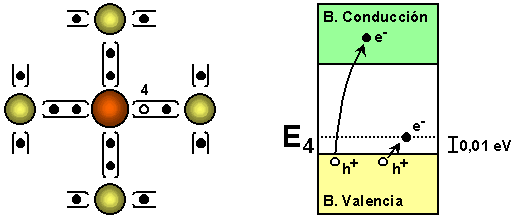
\includegraphics[scale=0.45]{../figs/Semiconductor_tipo_p}

}\subfloat[Semiconductor tipo n.\label{fig:Semiconductor-tipo-n}]{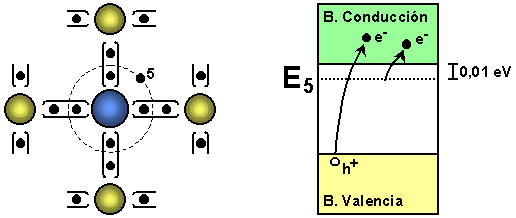
\includegraphics[scale=0.45]{../figs/Semiconductor_tipo_n}

}

\caption{Semiconductores dopados.}



\end{figure}


Supongamos ahora la existencia de dos semiconductores, uno tipo p
y otro tipo n (figura \ref{fig:Uni=0000F3n-p-n}). Al unirlos físicamente
se produce un desequilibrio dada la diferente concentración de electrones
y huecos en cada cristal. Para alcanzar el equilibrio se produce la
difusión de portadores mayoritarios, de forma que aparece un movimiento
de huecos desde el cristal p al cristal n, quedando aquel cargado
negativamente. Simultáneamente existe un movimiento de electrones
desde el cristal n a cristal p, quedando aquel cargado positivamente.
Si los huecos y electrones no fuesen partículas cargadas, este proceso
de difusión continuaría hasta alcanzar una concentración uniforme
en todo el volumen. Pero la carga de los portadores de los iones que
permanecen ligados a la red impide que el proceso de difusión se desarrolle
totalmente. 

Los iones cargados son el origen de un campo eléctrico orientado desde
el semiconductor n (cargado positivamente) hacia el semiconductor
p (cargado negativamente). Este campo arrastra a los electrones del
cristal p hacia el n, y expulsa a los huecos desde el cristal n hacia
el p. La dirección de este proceso de arrastre es precisamente la
contraria al proceso de difusión. El equilibrio se alcanza cuando
los movimientos de difusión y de arrastre se compensan. En el equilibrio
los portadores minoritarios (huecos en el cristal n y electrones en
el cristal p) que atraviesan la unión se recombinan, de forma que
los electrones que provienen del cristal n forman enlaces con los
huecos del cristal p y viceversa. Esta recombinación se produce en
la zona cercana a la unión, denominada zona de carga de espacio. Esta
región queda despoblada de portadores y habitada sólo por iones cargados
ligados a la red que generan un campo eléctrico de arrastre en la
unión. Este campo eléctrico supone la existencia de una barrera de
potencial%
\footnote{El valor de este salto es inferior a la anchura de la banda prohibida
de los semiconductores que participan en la unión%
} que recibe el nombre de potencial termodinámico y que impide el paso
de los portadores mayoritarios de uno a otro cristal. Así, una vez
alcanzado el equilibrio en una unión p-n, la corriente eléctrica es
nuevamente nula.

%
\begin{figure}
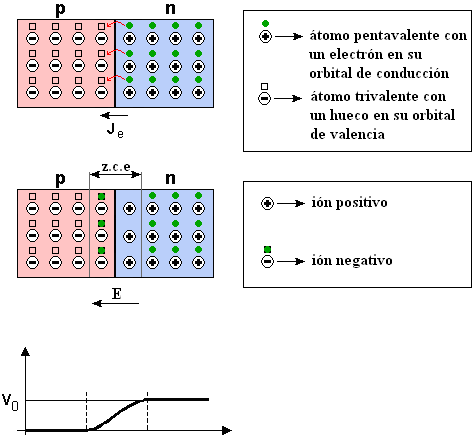
\includegraphics[scale=0.5]{../figs/Diodo_pn_-_zona_de_carga_espacial}

\caption{Unión p-n.\label{fig:Uni=0000F3n-p-n}.}



\end{figure}


Para conseguir la circulación de corriente a través de esta unión
p-n es necesario romper el equilibrio alcanzado y reducir el valor
del potencial termodinámico. La solución consiste en polarizar la
unión p-n. Si aplicamos una diferencia de potencial entre los extremos
del cristal de forma que el lado p adquiera una tensión positiva respecto
al lado n, diremos que la unión p-n está polarizada en directa. En
estas condiciones se reduce la barrera de potencial y, en consecuencia
el valor del campo eléctrico de la zona de unión. Por ello, la corriente
de arrastre disminuye y no puede compensar la corriente de difusión.
El equilibrio ya no existe y aparece un flujo neto de corriente. Los
huecos del lado p pueden ahora atravesar la zona de carga de espacio
y son inyectados en la zona n, donde son portadores minoritarios.
Aquí, aparecerá un exceso de huecos respecto del equilibrio y por
tanto se originará un proceso de difusión y recombinación. Lo mismo
puede decirse de los electrones de la zona n. Así, aparecen dos corrientes
en sentidos contrarios pero, dado que se trata de partículas de diferente
signo, las dos corrientes no se anulan entre sí y dan origen a una
corriente total aprovechable. El criterio convencional en electricidad
toma como sentido de la corriente el debido a las cargas positivas,
y por tanto la corriente entra en la unión por la zona p y sale por
la zona n.

Si la diferencia de potencial aplicada consigue que la zona p esté
a menor tensión que la zona n, la unión queda polarizada en inversa.
En estas condiciones la barrera de potencial en la unión queda reforzada
y el paso de portadores de una a otra zona queda aún más debilitado.
Así, la corriente que atraviesa la unión en polarización inversa es
de muy bajo valor.

El dispositivo electrónico basado en una unión p-n se denomina diodo.
La zona p del diodo es el ánodo y la zona n es el cátodo. La característica
tensión-corriente de este dispositivo queda recogida en la ecuación
de Shockley (ecuación \ref{eq:EcuacionDiodo}) y representada en la
figura \ref{fig:EcuacionDiodo}:\begin{equation}
I_{D}=I_{0}\cdot[\exp(\frac{V}{m\cdot V_{T}})-1]\label{eq:EcuacionDiodo}\end{equation}
\nomenclature[Id]{$I_{D}$}{Corriente de diodo de una célula}donde
$I_{0}$\nomenclature[I0]{$I_{0}$}{corriente de saturación en oscuridad del diodo}
es la corriente de saturación en oscuridad del diodo, $V$ la tensión
aplicada al diodo (considerada positiva cuando el valor en el ánodo
es superior al del cátodo) y $m$\nomenclature[m]{$m$}{Factor de idealidad del modelo de un diodo}
el factor de idealidad del diodo. Este factor puede tomar valores
entre 1 y 2, y se emplea para ajustar la ecuación \ref{eq:EcuacionDiodo}
al funcionamiento real del diodo. Para una temperatura ambiente de
$\SI{300}{\kelvin}$, $V_{T}=\frac{\mathrm{k}T}{\mathrm{e}}=\SI{25.85}{\milli\volt}$\nomenclature[Vt]{$V_{T}$}{Potencial térmico},
conocido como potencial térmico, donde $\mathrm{k}$\nomenclature[k]{$k$}{Constante de Boltzmann}
es la constante de Boltzmann, $T$ la temperatura del diodo (en grados
Kelvin), y $\mathrm{e}$ es la carga del electrón. Como se observa
en la figura, cuando la polarización del diodo es directa, la corriente
que circula por él crece de forma exponencial, pero permanece cercana
a cero ($I_{0}$) cuando la polarización es inversa. El símbolo empleado
para representar este dispositivo obedece a este funcionamiento (figura
\ref{fig:DiodoPolarizadoDirecta}).

%
\begin{figure}
\subfloat[Característica corriente-tensión de un diodo según la
ecuación \ref{eq:EcuacionDiodo}.\label{fig:EcuacionDiodo}]{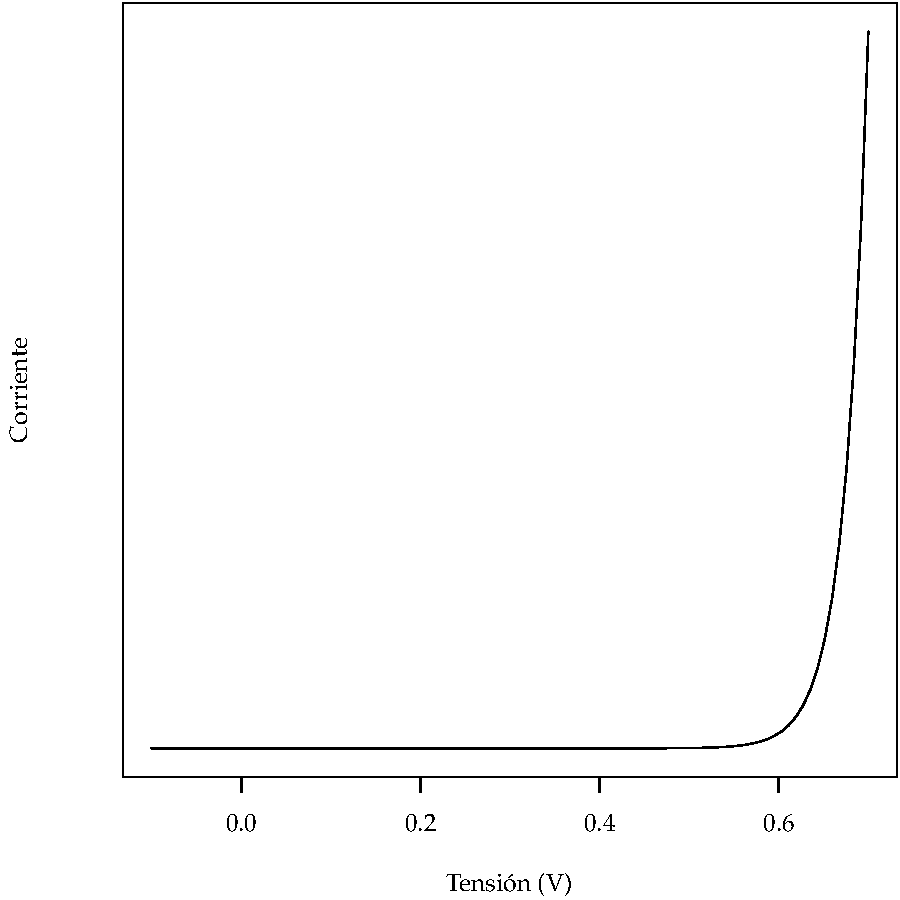
\includegraphics[scale=0.4]{../figs/EcuacionDiodo}}

\subfloat[Diodo polarizado en directa.\label{fig:DiodoPolarizadoDirecta}]{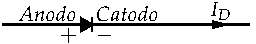
\includegraphics[scale=0.7]{../figs/Diodo}}

\caption{Representación y comportamiento de un diodo.}

\end{figure}



\subsection{La unión P-N iluminada}

\nocite{Wenham.Green.ea2000,Lorenzo2006c}

En 1905 Albert Einstein, en un artículo titulado {}``Un punto de
vista heurístico sobre la producción y transformación de la luz''
exponía la tesis de que la emisión de electrones era producida por
la absorción de cuantos de luz que más tarde serían llamados fotones.
Este efecto fotoeléctrico había sido previamente observado por Heinrich
Hertz en 1887, y analizado sucesivamente por Joseph John Thomson en
1889, y Philipp von Lenard en 1902. 

Einstein mostró como la idea de partículas discretas de luz podía
explicar el efecto fotoeléctrico y la presencia de una frecuencia
característica para cada material por debajo de la cual no se producía
ningún efecto. El trabajo de Einstein predecía que la energía con
la que los electrones escapaban del material aumentaba linealmente
con la frecuencia de la luz incidente. Sorprendentemente este aspecto
no había sido observado en las experiencias anteriores. La demostración
experimental de este aspecto fue llevada a cabo en 1915 por el físico
estadounidense Robert Andrews Millikan (\url{http://es.wikipedia.org/wiki/Efecto_fotoeléctrico}). 

La energía de un fotón se cuantifica mediante la ecuación \ref{eq:EnergiaFoton}:\begin{equation}
E_{f}=\frac{h\cdot c}{\lambda}\label{eq:EnergiaFoton}\end{equation}
\nomenclature[Ef]{$E_{f}$}{Energía de un fotón}siendo $h$ la constante
de Planck, $c$ la velocidad de la luz en el vacío y $\lambda$\nomenclature[lambda]{$\lambda$}{Longitud de onda de un fotón}
la longitud de onda del fotón%
\footnote{La frecuencia del fotón es $f=\frac{c}{\lambda}$%
}. Es importante resaltar que intensidad de la radiación incidente
influye en la cantidad de electrones generados pero no determina la
energía de estos electrones, energía que sólo depende de la frecuencia
fotónica. 

El efecto fotoeléctrico es el fundamento del funcionamiento de las
células solares, dispositivos basados en la unión p-n descrita anteriormente,
cuyos electrones se desplazan a la banda de conducción por el aporte
energético de fotones incidentes. El campo eléctrico de la unión conduce
los portadores generados por esta interacción y dificulta la recombinación.
Esta corriente de iluminación, denominada fotocorriente, es ahora
aprovechable por un circuito externo. Sin embargo, la presencia de
tensión en los terminales de la unión (por ejemplo, la diferencia
de potencial en una resistencia alimentada por el dispositivo) reduce
la barrera de potencial de la unión, y consecuentemente favorece los
procesos de recombinación que, como fue descrito anteriormente, constituyen
la corriente del diodo, que ahora se denomina corriente de oscuridad.
Consecuentemente, en una unión p-n iluminada coexisten dos corrientes
de sentido contrapuesto y con orígenes diferentes. La corriente de
iluminación o fotocorriente, debida a la incidencia de fotones, circula
desde la región n a la región p. La corriente de oscuridad o corriente
de diodo, debida a la recombinación de portadores favorecida por la
tensión en el circuito externo, circula desde la región p hacia la
n (figura \ref{fig:EsquemaCorrientesCelula}). La corriente total
se expresa mediante la ecuación \ref{eq:CorrienteCelula}: \begin{equation}
I=I_{L}-I_{0}\cdot[\exp(\frac{V}{m\cdot V_{T}})-1]\label{eq:CorrienteCelula}\end{equation}
\nomenclature[Il]{$I_{L}$}{Corriente de iluminación de una célula}\nomenclature[I]{$I$}{Corriente neta de una célula}\nomenclature[V]{$V$}{Tensión en una célula}

En esta ecuación se emplea $I_{L}$ para designar a la fotocorriente
y, dado que el aprovechamiento de la célula solar consiste en extraer
esta corriente al exterior, se ha utilizado el signo negativo para
la corriente de diodo.


\begin{figure}
\begin{centering}
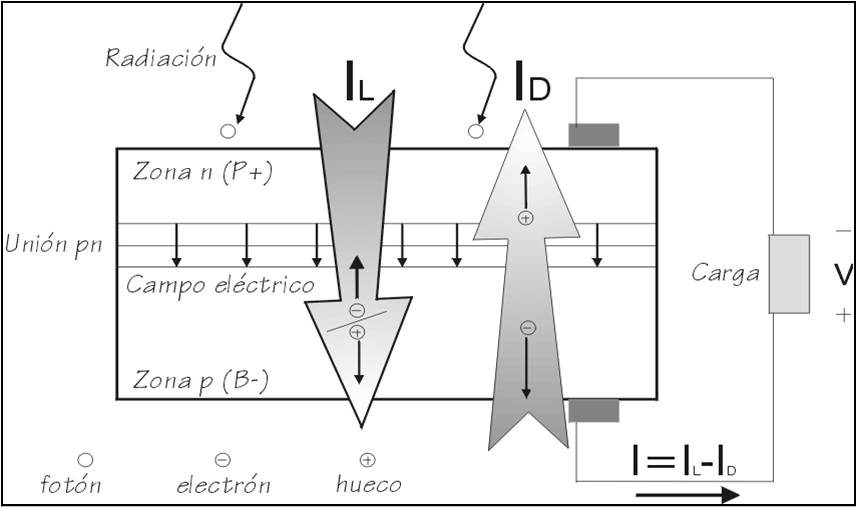
\includegraphics[scale=0.7]{../figs/CelulaSolar}
\end{centering}

\caption{Corriente de iluminación y corriente de diodo en una célula solar
que alimenta a una carga.\label{fig:EsquemaCorrientesCelula}}

\end{figure}


El fenómeno de generación de portadores debido al efecto fotoeléctrico
depende de la frecuencia de los fotones incidentes. Si el fotón incidente
es poco energético respecto a las características de la unión p-n
($E_{f}<E_{g}$), no interactúa con el semiconductor y lo atraviesa
como si fuese transparente. Los fotones más energéticos (aquellos
con baja longitud de onda y alta frecuencia) provoca la rotura de
un enlace en la superficie del semiconductor. El par electrón-hueco
producido se encuentra lejos del campo eléctrico de la unión, de forma
que éste no podrá ejercer sobre ellos la fuerza adecuada para evitar
que se recombinen antes de salir del semiconductor al circuito exterior.
De forma intuitiva se comprende que la unión p-n podrá aprovechar
adecuadamente aquellos fotones suficientemente energéticos para provocar
la rotura de un enlace, pero no tanto como para que esta interacción
se realice demasiado lejos de la unión. Para el silicio son aprovechables
los fotones en el espectro visible ($\SI{400}{\nano\meter}<\lambda<\SI{700}{\nano\meter}$)
y ultravioleta cercano ($\SI{300}{\nano\meter}<\lambda<\SI{400}{\nano\meter}$).
Sin embargo, los fotones que pertenecen al infrarrojo ($\lambda>\SI{1100}{\nano\meter}$)
no consiguen romper enlaces y los del ultravioleta son demasiado energéticos
(figura \ref{fig:EsquemaPerdidasCelula}).


%
\begin{figure}
\begin{centering}
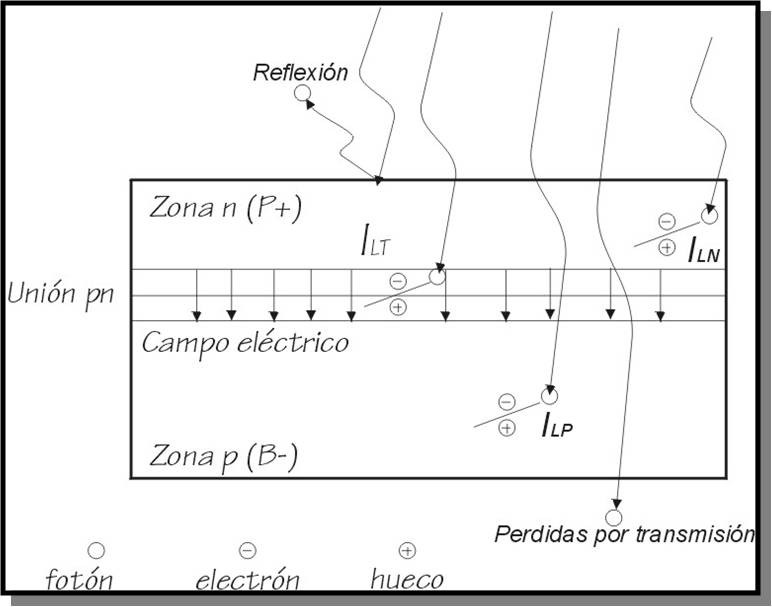
\includegraphics[scale=0.75]{../figs/CelulaSolar2}
\end{centering}

\caption{Pérdidas de transmisión, reflexión y recombinación en una célula solar.\label{fig:EsquemaPerdidasCelula}}

\end{figure}



Los fotones con $E_{f}<E_{g}$ atraviesan el cristal sin ser absorbidos
y son cuantificados mediante las pérdidas de no-absorción. Debido
a la anchura finita del semiconductor y su coeficiente de absorción,
parte de los fotones con $E_{f}>E_{g}$ no son absorbidos y constituyen
las pérdidas de transmisión. Aquellos que son absorbidos pero se recombinan
dentro del dispositivo componen las pérdidas por recombinación. Por
último, la diferencia entre los índices de refracción del aire y el
dispositivo provoca las pérdidas por reflexión. Para reducir las pérdidas
reflexión se recurre a capas que adaptan los dos índices de refracción,
y al texturado de la superficie para conseguir que el rayo de luz
reflejado vuelva a introducirse en el material.

Suponiendo conocido el número de fotones incidentes por unidad de
área para cada energía, $S(E)$, y el área del dispositivo, $A$,
la ecuación \ref{eq:Fotocorriente} expresa que el dispositivo no
podrá aprovechar íntegramente el flujo fotónico incidente.

\begin{equation}
I_{L}<e\cdot A\cdot\intop_{E_{G}}^{\infty}S(E)\mathrm{d}E\label{eq:Fotocorriente}\end{equation}



\section{Funcionamiento de una célula solar}

Como describe la ecuación \ref{eq:CorrienteCelula}, la corriente
de una célula solar es un balance entre la fotocorriente y la corriente
de oscuridad que, a su vez, depende de la tensión aplicada en los
terminales del dispositivo. Esta relación se representa en la figura
\ref{fig:CurvaIVCelula}. Cuando la tensión aplicada es nula (la célula
está cortocircuitada) la corriente se debe exclusivamente a la fotocorriente.
El valor de la corriente permanece casi constante hasta las cercanías
del valor de tensión en el que el diodo comienza a conducir (figura
\ref{fig:EcuacionDiodo}). A partir de este punto, la corriente disminuye
abruptamente hasta alcanzar un valor nulo (célula en circuito abierto)
en el punto donde la fotocorriente y la corriente de oscuridad quedan
compensadas. 


%
\begin{figure}
\begin{centering}
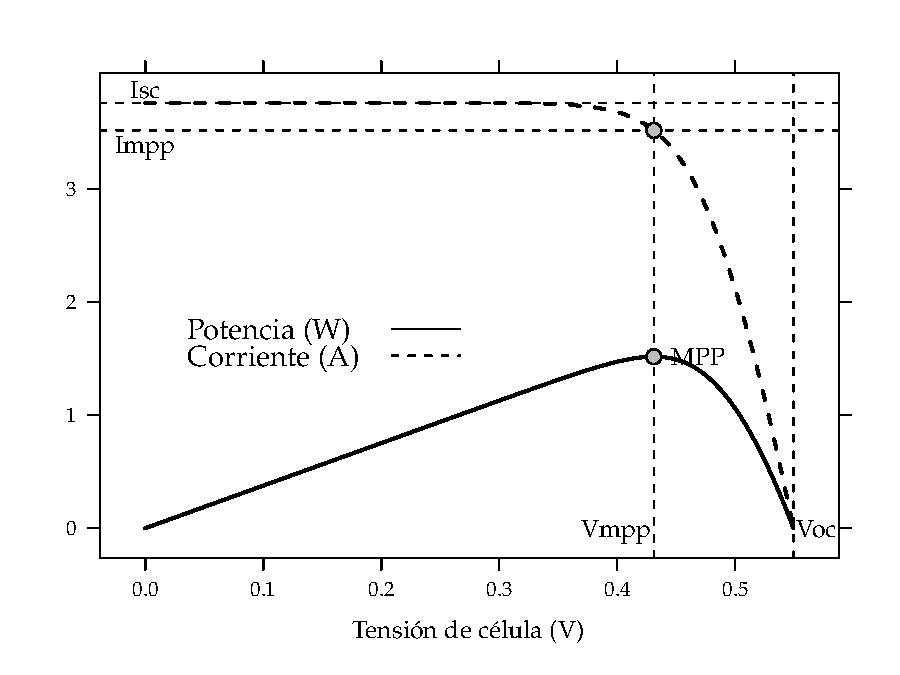
\includegraphics[scale=0.75]{../figs/CurvaIV_Ta20_G800}
\end{centering}

\caption{Curvas corriente-tensión (línea discontinua) y potencia-tensión (línea
continua) de una célula solar ($T_a=\SI{20}{\celsius}$ y $G=\SI{800}{\watt\per\meter\squared}$).\label{fig:CurvaIVCelula}}

\end{figure}



Los dos puntos extremos de cortocircuito y circuito abierto quedan
definidos con dos parámetros, la corriente de cortocircuito, $I_{sc}$,
y la tensión de circuito abierto, $V_{oc}$\nomenclature[Isc]{$I_{sc}$}{Corriente de cortocircuito de una célula}\nomenclature[Voc]{$V_{oc}$}{Tensión de circuito abierto de una célula}.
La corriente de cortocircuito es fácilmente calculable a partir de
la ecuación \ref{eq:CorrienteCelula} sin más que imponer $V=0$:

\begin{equation}
I_{sc}=I(V=0)=I_{L}\label{eq:Isc}\end{equation}
mientras que la tensión de circuito abierto se deduce con la condición
$I=0$:

\begin{equation}
V_{oc}=V(I=0)=m\cdot\frac{k\cdot T_{c}}{e}\cdot\ln\left(\frac{I_{L}}{I_{0}}+1\right)\label{eq:Voc}\end{equation}


Estos dos parámetros suelen estar disponibles en la información asociada
a una célula. Será conveniente reescribir la ecuación \ref{eq:CorrienteCelula}
para incluirlos y obtener la ecuación \ref{eq:EcuacionCelulaInicial}:

\begin{equation}
I=I_{sc}\cdot\left[1-\exp\left(\frac{e\cdot(V_{oc}-V)}{m\cdot k\cdot T_{c}}\right)\right]\label{eq:EcuacionCelulaInicial}\end{equation}



\subsection{Punto de máxima potencia}

Superpuesta a la curva corriente-tensión, la figura \ref{fig:CurvaIVCelula}
incluye la relación entre la potencia y la tensión. Es evidente la
presencia de un máximo que adquiere el nombre de punto de máxima potencia
(\emph{MPP, maximum power point }en sus siglas inglesas). La localización
de este punto viene definida por la condición $\frac{\mathrm{d}P}{\mathrm{d}V}=0$.
La potencia entregada por la célula en este punto será la considerada
como potencia nominal, $P_{mpp}=I_{mpp}\cdot V_{mpp}$\nomenclature[MPP]{MPP}{Punto de máxima potencia de un dispositivo fotovoltaico}\nomenclature[Impp]{$I_{mpp}$}{Corriente de una célula en el punto de máxima potencia}\nomenclature[Vmpp]{$V_{mpp}$}{Tensión de una célula en el punto de máxima potencia}\nomenclature[Pmpp]{$P_{mpp}$}{Potencia máxima de una célula}.
Las unidades de esta potencia son vatios pico (Wp), reflejando la
idea de potencia máxima alcanzable.

Dado que la célula funciona en corriente continua, su potencia es
$P=V\cdot I$ y por tanto:

\begin{eqnarray}
\frac{\mathrm{d}(I\cdot V)}{\mathrm{d}V} & = & V\cdot\frac{\mathrm{d}I}{\mathrm{d}V}+I\cdot\frac{\mathrm{d}V}{\mathrm{d}V}\nonumber \\
\mathrm{d}P & = & V\cdot\mathrm{d}I+I\cdot\mathrm{d}V\end{eqnarray}


Antes de este punto, $\frac{\mathrm{d}P}{\mathrm{d}V}>0$ o, de
forma equivalente, $\frac{\mathrm{d}I}{\mathrm{d}V}>-\frac{I}{V}$.
Entre este punto y el circuito abierto $\frac{\mathrm{d}P}{\mathrm{d}V}<0$
o, de forma equivalente, $\frac{\mathrm{d}I}{\mathrm{d}V}<-\frac{I}{V}$.
En el punto de máxima potencia se cumplirá:\begin{equation}
\frac{\mathrm{d}I}{\mathrm{d}V}=-\frac{I_{mpp}}{V_{mpp}}\label{eq:MPP_derivada}\end{equation}



\subsection{Factor de forma y Eficiencia}

El área encerrada por el rectángulo definido por el producto $I_{mpp}\cdot V_{mpp}$
es, como es observable en la figura \ref{fig:CurvaIVCelula}, inferior
a la representada por el producto $I_{sc}\cdot V_{oc}$. La relación
entre estas dos superficies se cuantifica con el factor de forma:

\begin{equation}
FF=\frac{I_{mpp}\cdot V_{mpp}}{I_{sc}\cdot V_{oc}}\label{eq:FactorForma}\end{equation}
\nomenclature[FF]{$FF$}{Factor de forma de un dispositivo fotovoltaico}

El factor de forma es tanto más cercano a la unidad cuánto mas acentuado
sea el codo localizado en el punto de máxima potencia. Su valor, normalmente
comprendido entre $0.7$ y $0.8$, varía poco de unas células a otros.
Conociendo los valores de $I_{sc}$ y $V_{oc}$ es posible calcular
la potencia en el punto de máxima potencia, dado que $P_{mpp}=FF\cdot I_{sc}\cdot V_{oc}$.

Por otra parte, la calidad de una célula se puede cuantificar con
la eficiencia de conversión según la ecuación \ref{eq:EficienciaCelula}

\begin{equation}
\eta=\frac{I_{mpp}\cdot V_{mpp}}{P_{L}}\label{eq:EficienciaCelula}\end{equation}
donde $P_{L}$ representa la potencia luminosa que incide en la célula.
Como es evidente de la ecuación \ref{eq:EficienciaCelula}, este valor
de eficiencia se corresponde al caso en el que el acoplamiento entre
la carga y la célula permite a ésta trabajar en el punto de máxima
potencia. En la figura \ref{fig:EvolucionEficienciaC=0000E9lulas}
se muestra la evolución temporal del valor de eficiencia de célula
de laboratorio para diferentes tecnologías. Las células industriales
de silicio suelen ofrecer eficiencias comprendidas entre el 13\% y
el 17\%.

%
\begin{figure}
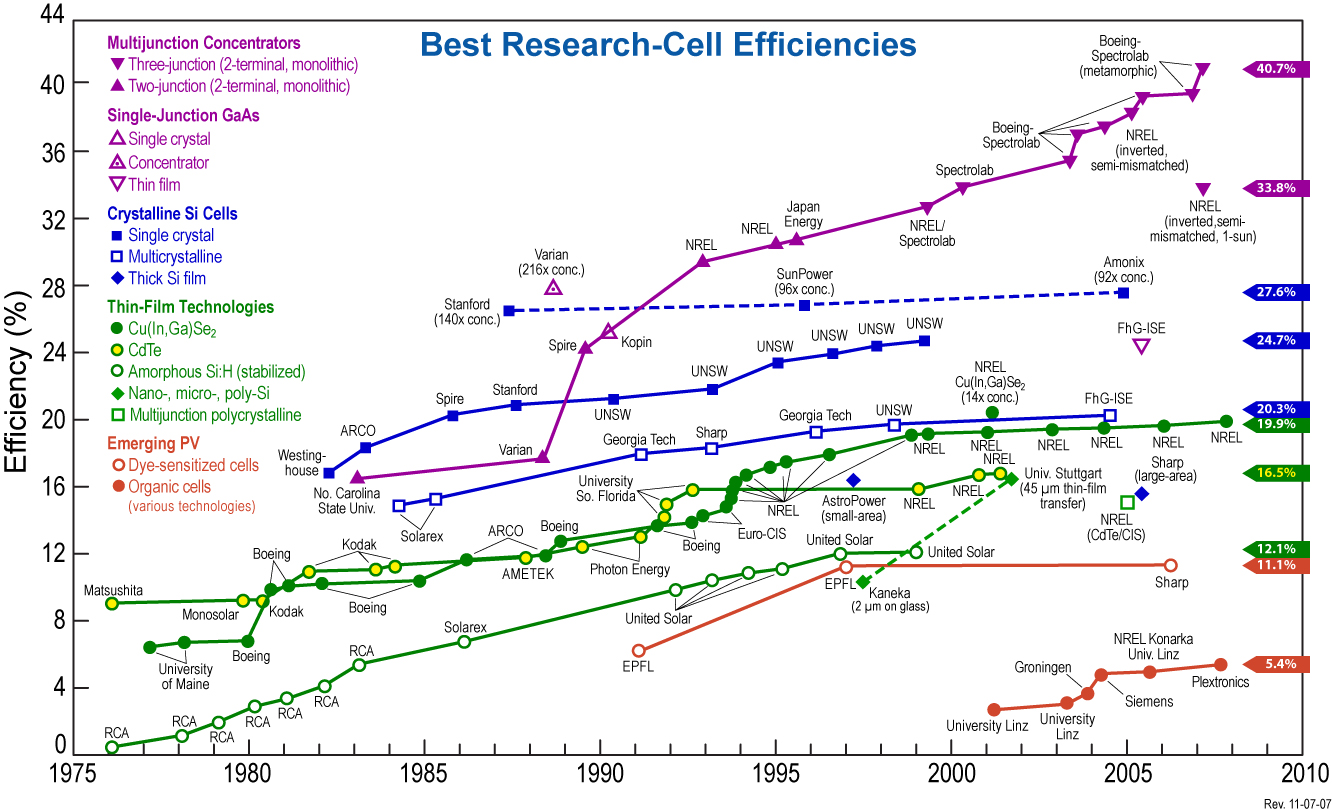
\includegraphics[scale=0.35]{../figs/PVeff(rev110707)d}\caption{Evolución de la eficiencia de células según la tecnología (según el
National Renewable Energy Laboratory (EEUU).\label{fig:EvolucionEficienciaC=0000E9lulas}}

\end{figure}



\subsection{Circuito equivalente de una célula solar}

Para analizar el comportamiento de una célula en un circuito es conveniente
emplear modelos equivalentes alternativos a la ecuación \ref{eq:EcuacionCelulaInicial}.
La corriente fotogenerada puede ser modelada con un generador de corriente
mientras que la corriente de oscuridad puede ser representada con
un diodo, tal y como se recoge en la figura \ref{fig:M=0000F3deloCelula}.
En esta figura se incluyen una resistencia serie y una resistencia
paralelo para efectos no incluidos en la ecuación \ref{eq:EcuacionCelulaInicial}
pero apreciables en las células reales. Teniendo en cuenta estas dos
resistencias se obtiene:

\begin{equation}
I=I_{L}-I_{0}\cdot[\exp(\frac{V+I\cdot R_{s}}{m\cdot V_{T}})-1]-\frac{V+I\cdot R_{s}}{R_{p}}\label{eq:CorrienteCelulaRsRp}\end{equation}
\nomenclature[Rs]{$R_{s}$}{Resistencia serie de una célula solar}\nomenclature[Rp]{$R_{p}$}{Resistencia paralelo de una célula solar}

La resistencia serie representa la resistencia debida a los contactos
metálicos con el semiconductor, a las capas semiconductoras y a la
malla de metalización. Esta resistencia reduce principalmente el factor
de forma y, en menor medida, la corriente de cortocircuito. En la
figura \ref{fig:EfectoRs} se comprueba que valores altos de la resistencia
serie alteran la pendiente de la curva I-V en la región comprendida
entre el MPP y la tensión de circuito abierto y reducen el valor de
potencia en el MPP.

%
\begin{figure}
\hfill{}\subfloat[Curva I-V.]{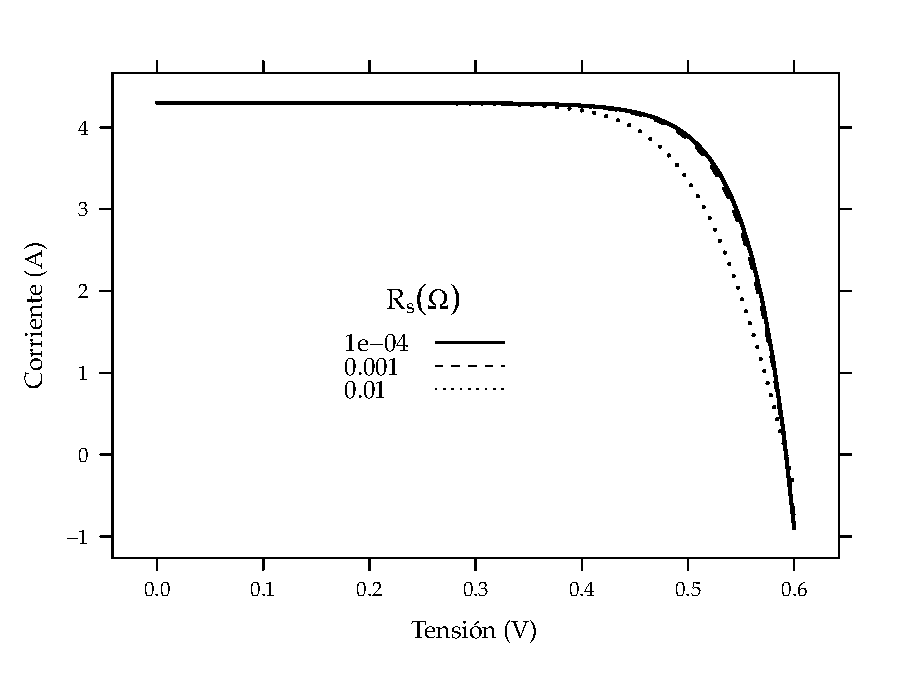
\includegraphics[scale=0.5]{../figs/InfluenciaRs_IV}

}\hfill{}\subfloat[Curva P-V.]{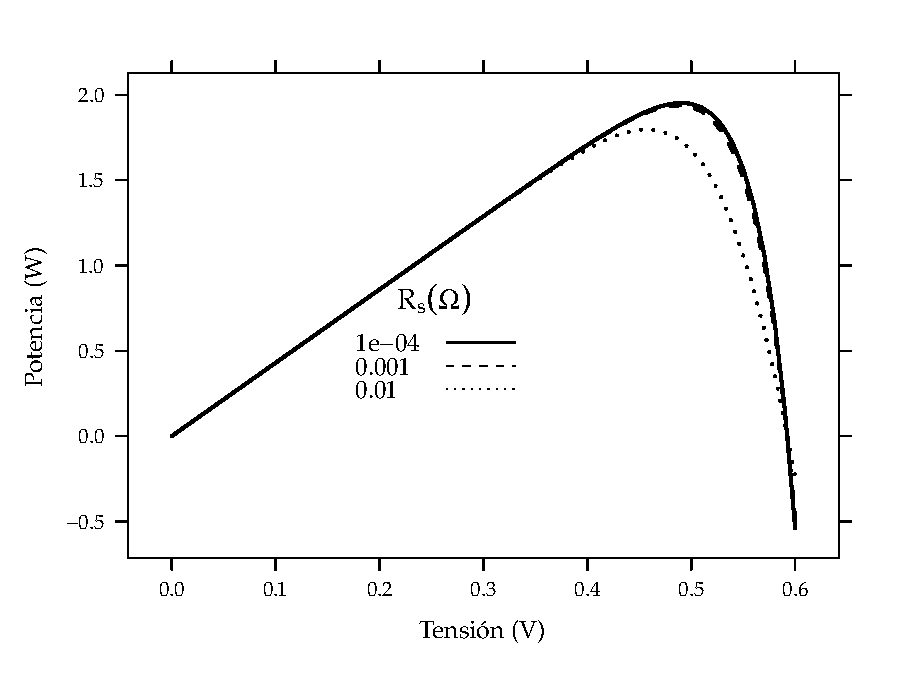
\includegraphics[scale=0.5]{../figs/InfluenciaRs_Potencia}

}\hfill{}

\caption{Efecto de la resistencia serie en las curvas I-V y P-V.\label{fig:EfectoRs}}



\end{figure}


La resistencia paralelo representa las fugas de corriente en los bordes
de célula, los posibles cortocircuitos metálicos y la recombinación
favorecida en las fronteras de grano del cristal. Esta resistencia
reduce el factor de forma y la tensión de circuito abierto. En la
figura \ref{fig:EfectoRsh} se comprueba que valores bajos de la resistencia
paralelo alteran la pendiente de la curva I-V en la región comprendida
entre el cortocircuito y el MPP y reducen el valor de potencia en
el MPP. En general, toma valores suficientemente altos como para que
su influencia en el funcionamiento global sea baja, y de ahí que frecuentemente
se desprecie su contribución. 

%
\begin{figure}
\hfill{}\subfloat[Curva I-V.]{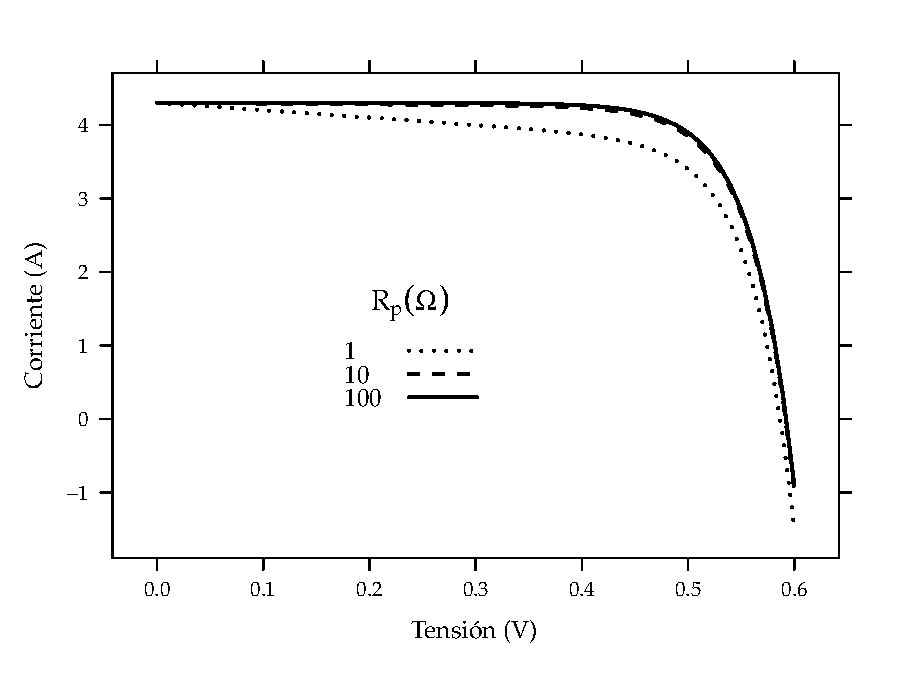
\includegraphics[scale=0.5]{../figs/InfluenciaRsh_IV}

}\hfill{}\subfloat[Curva P-V.]{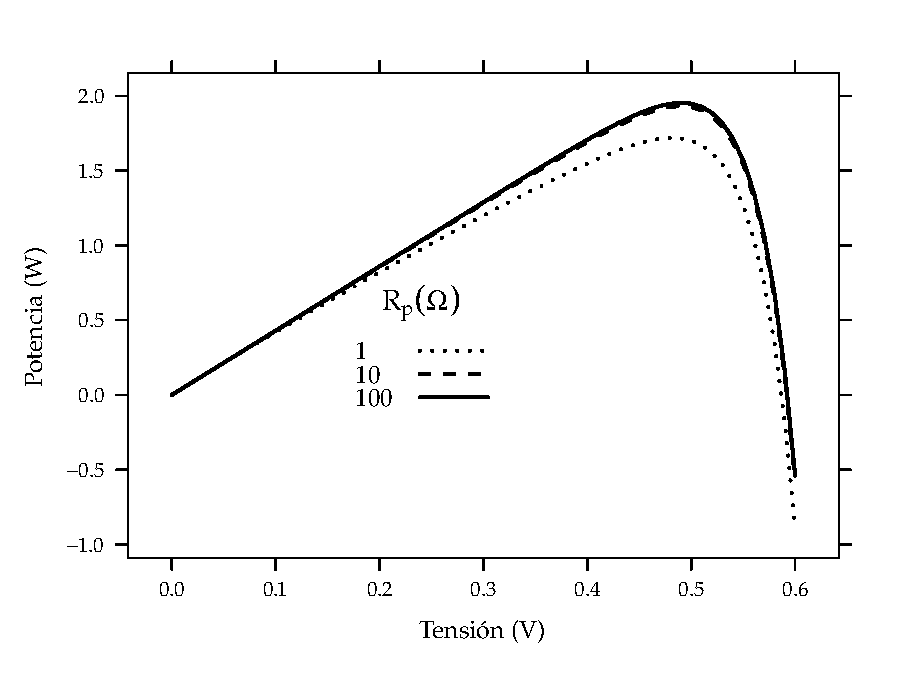
\includegraphics[scale=0.5]{../figs/InfluenciaRsh_Potencia}

}\hfill{}

\caption{Efecto de la resistencia paralelo en las curvas I-V y P-V.\label{fig:EfectoRsh}}

\end{figure}


Considerando que el valor de la exponencial es notablemente superior
a 1 en todas las condiciones de operación, que la contribución de
la resistencia paralelo es despreciable y que la corriente de cortocircuito
es equivalente a la corriente fotogenerada, obtenemos la ecuación
\ref{eq:CorrienteCelulaRs}: \begin{equation}
I=I_{sc}-I_{0}\cdot\exp(\frac{V+I\cdot R_{s}}{m\cdot V_{T}})\label{eq:CorrienteCelulaRs}\end{equation}


De esta ecuación podemos obtener otra expresión para la tensión de
circuito abierto:\begin{equation}
V_{oc}=m\cdot V_{t}\cdot\ln(\frac{I_{sc}}{I_{o}})\end{equation}
y por tanto:\begin{equation}
I_{0}=I_{sc}\cdot\exp(-\frac{V_{oc}}{m\cdot V_{t}})\end{equation}


Sustituyendo estas expresiones en la ecuación \ref{eq:CorrienteCelulaRs}
obtenemos la ecuación que emplearemos como curva característica de
la célula solar: \begin{equation}
I=I_{sc}[1-\exp(\frac{V-V_{oc}+I\cdot R_{s}}{m\cdot V_{t}})]\label{eq:EcuacionCelulaFinal}\end{equation}
%
\begin{figure}
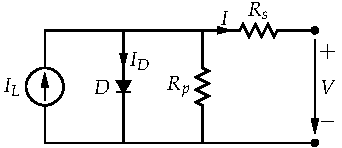
\includegraphics{../figs/ModeloElectricoCelulaSolar}\caption{Modelo eléctrico de una célula solar.\label{fig:M=0000F3deloCelula}}

\end{figure}



\subsection{Influencia de la temperatura y la radiación}

Para comprender correctamente el funcionamiento de la célula solar,
es preciso tomar en consideración la influencia de los dos principales
factores externos: la temperatura ambiente y la iluminación incidente.

El aumento de la temperatura ambiente a la que se encuentra la célula
estrecha el salto entre banda de valencia y conducción de forma que,
en condiciones de iluminación constante, aumenta \emph{ligeramente}
la fotocorriente. En general, esta relación es despreciable. Sin embargo,
el efecto en la tensión es más importante. El aumento en la temperatura
reduce la tensión de circuito abierto según el valor de
$dV_{oc}/dT_{c}$. 
donde $T_{c}$ es la temperatura de la célula, dependiente de la temperatura
ambiente y la irradiación incidente. La forma de calcular esta temperatura
de célula depende de las características constructivas del módulo
que encapsula a la célula. Si no hay información específica por parte del
fabricante, para células de silicio cristalino es habitual emplear el valor:
\begin{equation}
dV_{oc}/dT_{c} = \SI{-2.3}{\milli\volt\per\celsius}
\label{eq:VocTemperatura}
\end{equation}
\nomenclature[Tc]{$T_{c}$}{Temperatura de funcionamiento de una
  célula}

También disminuye el factor de forma y la eficiencia, ésta según la
relación $d\eta/dT_{c}=\SI{-0.4}{\percent\per\celsius}$
\nomenclature[eta]{$\eta$}{Eficiencia de una célula solar}.
El efecto de la temperatura en la curva característica queda recogido
en la figura \ref{fig:EfectoTemperatura}.


%
\begin{figure}
\begin{centering}
\subfloat[Curva I-V.]{\begin{centering}
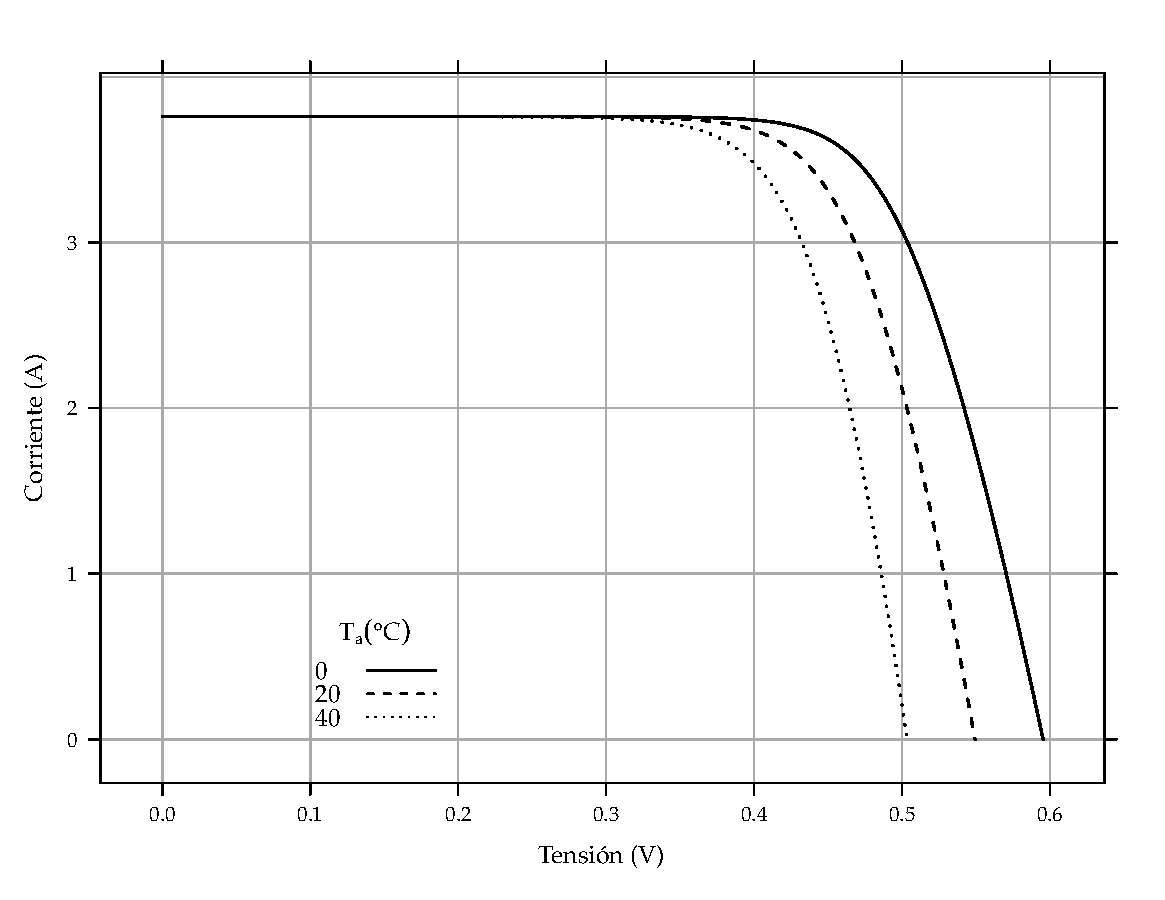
\includegraphics[scale=0.7]{../figs/CurvaIV_G800}
\par\end{centering}

}
\par\end{centering}

\begin{centering}
\subfloat[Curva P-V.]{\begin{centering}
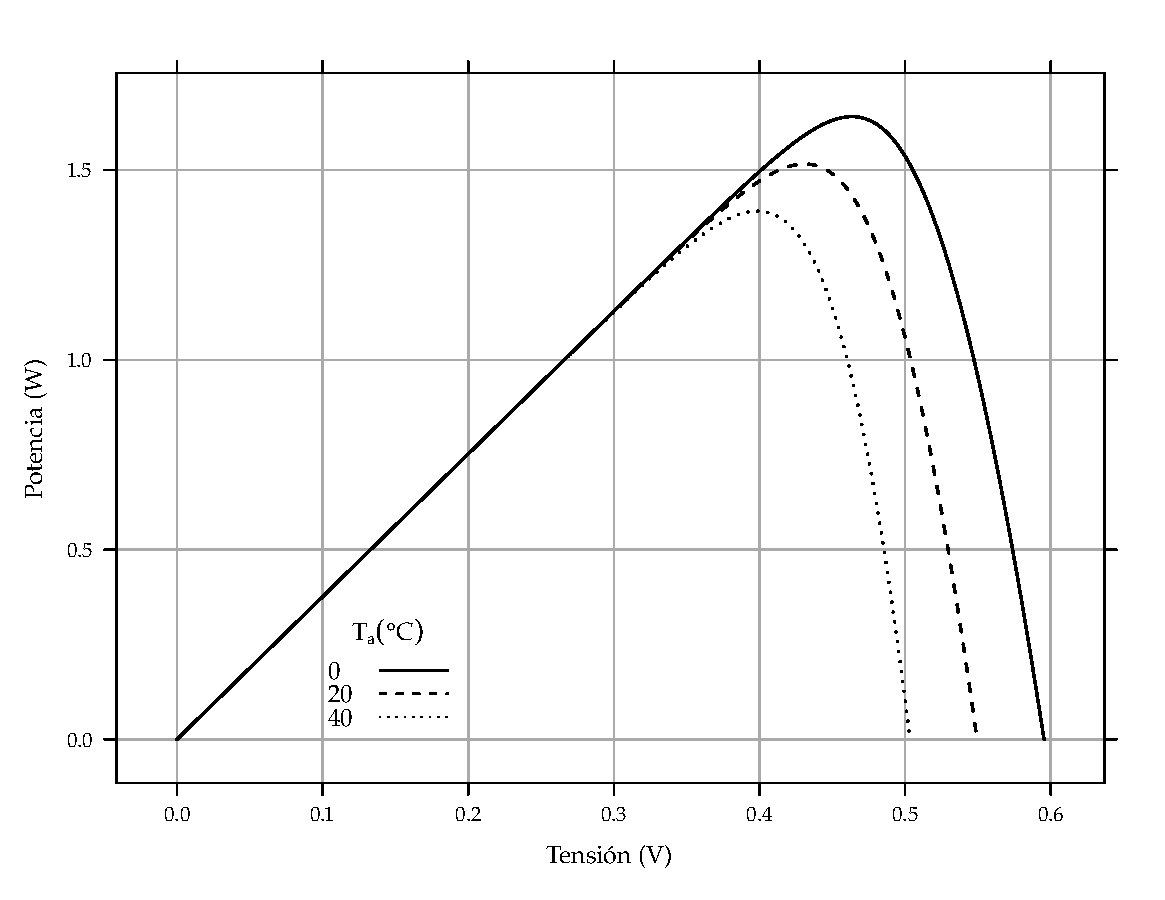
\includegraphics[scale=0.7]{../figs/CurvaPV_G800}
\par\end{centering}

}
\end{centering}

\caption{Efecto de la temperatura en la curva característica de una célula
solar ($G=\SI{800}{\watt\per\meter\squared}$).\label{fig:EfectoTemperatura}}

\end{figure}



En cuanto a la iluminación, es conveniente recordar que la fotocorriente
es proporcional a la intensidad de radiación (la cantidad de electrones
liberados dependía de la cantidad de fotones incidentes aprovechables),
$I_{L}(X)=X\cdot I_{L}(1)$, donde, empleando como referencia el nivel
de irradiancia denominado 1 Sol (equivalente a $\SI{1000}{\watt\per\meter\squared}$
con una masa de aire $AM=1$), se define $X$ como el factor de concentración
o nivel de irradiancia incidente en Soles. Por ejemplo, la fotocorriente
generada con $2$ soles, $I_{L}(2)$, será el doble de la generada
con 1 sol, $I_{L}(1)$. Recordando la ecuación \ref{eq:Isc}, \begin{eqnarray}
I_{sc}(X) & = & X\cdot I_{sc}(1)\label{eq:IscRadiacion}\end{eqnarray}


Si simbolizamos la tensión de circuito abierto a 1 Sol con $V_{oc1}$,
la dependencia de la tensión con la iluminación queda expresada mediante
una relación logarítmica, $V_{oc}=V_{oc1}+\frac{mkT_{c}}{e}\cdot\ln(X)$.
No obstante, el efecto de la irradiancia en la tensión de circuito
abierto es de menor importancia que en la corriente, y puede no ser
tenida en consideración en muchos casos prácticos. Por otra parte,
el factor de forma aumenta ligeramente con la irradiancia y la eficiencia
crece de forma logarítmica hasta alcanzar un nivel determinado por
las limitaciones físicas del dispositivo. El efecto de la irradiancia
en la curva característica queda recogido en la figura \ref{fig:EfectoIrradiancia}.


%
\begin{figure}
\begin{centering}
\subfloat[Curva I-V.]{\begin{centering}
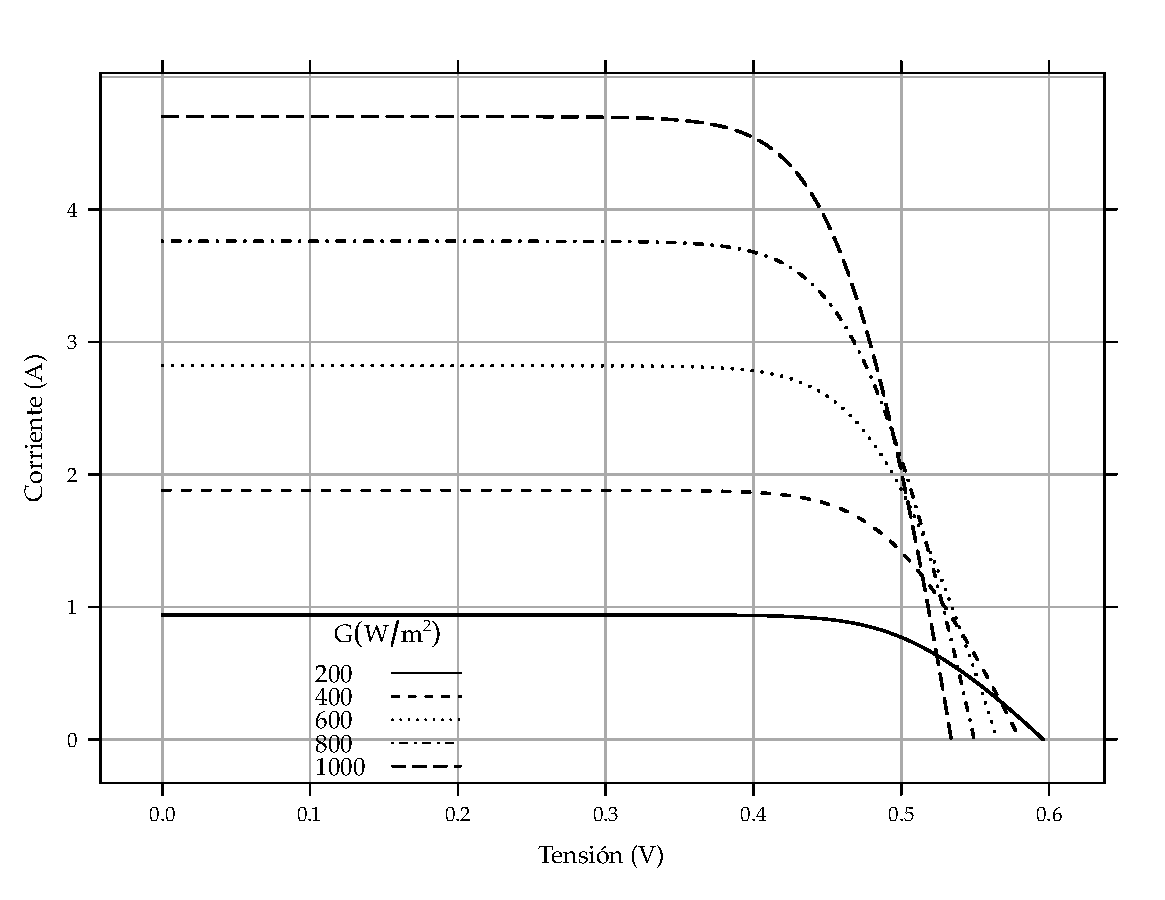
\includegraphics[scale=0.7]{../figs/CurvaIV_Ta20}
\par\end{centering}

}
\par\end{centering}

\begin{centering}
\subfloat[Curva P-V.]{\begin{centering}
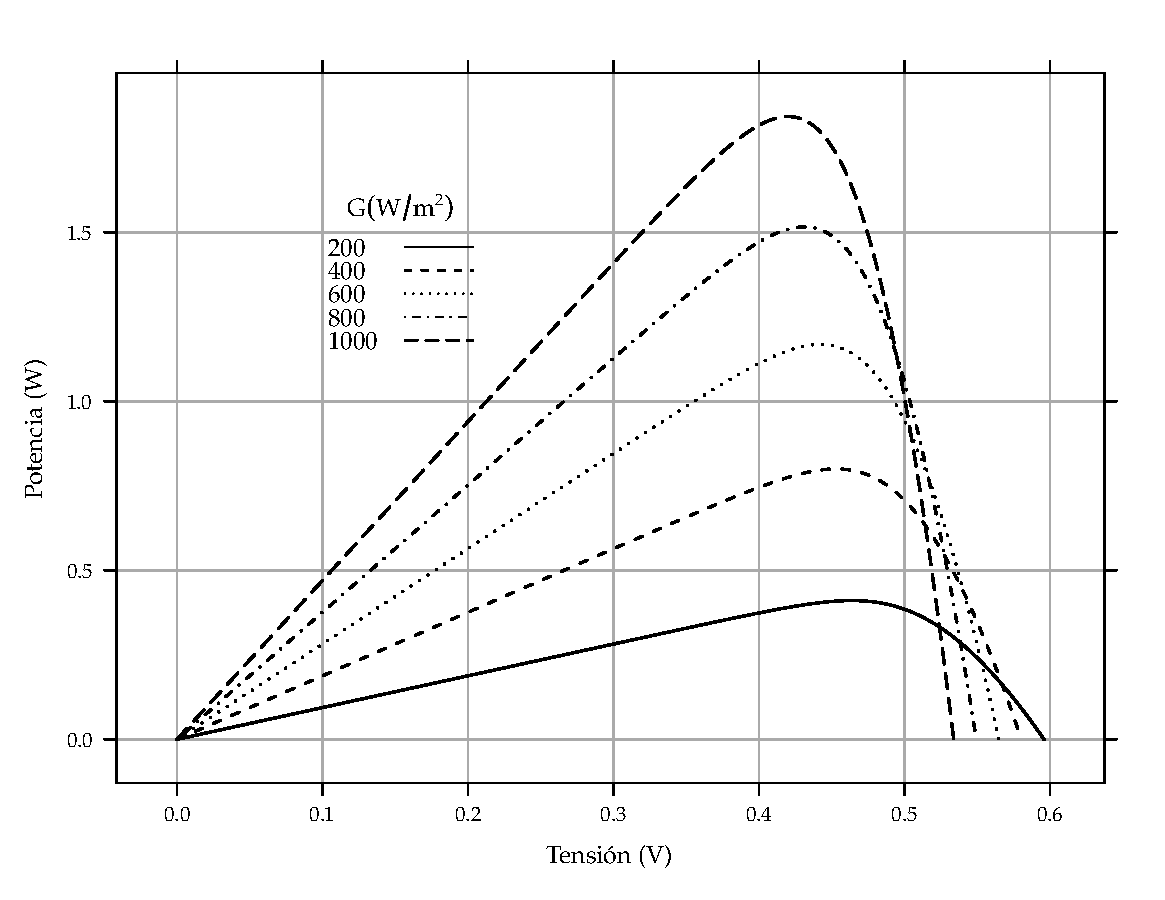
\includegraphics[scale=0.7]{../figs/CurvaPV_Ta20}
\par\end{centering}

}
\end{centering}

\caption{Efecto de la irradiancia en la curva característica de una célula
solar ($T_a=\SI{20}{\celsius}$).\label{fig:EfectoIrradiancia}}

\end{figure}



Tomando en cuenta estas influencias, se definen unas condiciones de
funcionamiento, denominadas condiciones estándar de medida (\emph{STC,
standard test conditions} en sus siglas inglesas), válidas para caracterizar
una célula en el entorno de un laboratorio. Esta condiciones vienen
determinadas por:
\begin{itemize}
\item Irradiancia: $G_{stc}=\SI{1000}{\watt\per\meter\squared}$ con incidencia
normal.  \nomenclature[Gstc]{$G_{stc}$}{Irradiancia incidente en condiciones estandar de medida}
\item Temperatura de célula: $T_{c}^{*}=\SI{25}{\celsius}$  \nomenclature[Tc*]{$T_{c}^{*}$}{Temperatura de célula en condiciones estándar de medida}\nomenclature[Impp*]{$I_{mpp}^{*}$}{Corriente de una célula en el punto de máxima potencia en condiciones estándar de medida}\nomenclature[Isc*]{$I_{sc}^{*}$}{Corriente de cortocircuito de una célula en condiciones estándar de medida}\nomenclature[Vmpp*]{$V_{mpp}^{*}$}{Tensión de una célula en el punto de máxima potencia en condiciones estándar de medida}\nomenclature[Voc*]{$V_{oc}^{*}$}{Tensión de circuito abierto de una célula en condiciones estándar de medida}
 \nomenclature[STC]{STC}{Condiciones estándar de medida de un dispositivo fotovoltaico}.
\item Masa de aire: $AM=1.5$
\end{itemize}
Es de uso común añadir un asterisco como superíndice para denotar
aquellos parámetros medidos en estas condiciones. Frecuentemente los
fabricantes informan de los valores de las tensiones $V_{oc}^{*}$
y $V_{mpp}^{*}$ y las corrientes $I_{sc}^{*}$ y $I_{mpp}^{*}$.
A partir de estos valores es posible referir a estas condiciones la
potencia, $P_{mpp}^{*}=I_{mpp}^{*}\cdot V_{mpp}^{*}$, el factor de
forma, $FF^{*}=\frac{P_{mpp}^{*}}{I_{sc}^{*}\cdot V_{oc}^{*}}$\nomenclature[FF*]{$FF^{*}$}{Factor de forma de una célula en condiciones estándar de medida}
y la eficiencia:

\begin{equation}
\eta^{*}=\frac{I_{mpp}^{*}\cdot V_{mpp}^{*}}{A\cdot G_{stc}}\label{eq:EficienciaCelula_STC}\end{equation}
\nomenclature[eta*]{$\eta^{*}$}{Eficiencia de una célula en condiciones estándar de medida}


\subsection{Cálculo del punto de máxima potencia\label{sub:CalculoMaximaPotencia}}

En el apartado anterior se ha puesto de manifiesto la relación entre
la temperatura y la irradiancia con la tensión de \emph{circuito abierto}
y la corriente de \emph{cortocircuito}. Además, es frecuente disponer
de los valores de la tensión y corriente en el punto de máxima potencia
en las condiciones estándar de medida. Para poder estimar el comportamiento
de la célula en otras condiciones, es necesario trasladar estos parámetros
a otros valores de temperatura e irradiancia.

El cálculo de la tensión y corriente en el punto de máxima potencia
a partir de la combinación entre la ecuación \ref{eq:MPP_derivada}
y la \ref{eq:EcuacionCelulaFinal} conduce a un sistema de ecuaciones
implícitas cuya resolución no es evidente. Una aproximación a esta
solución viene dada por la propuesta debida a J.M. Ruiz (según queda
recogida en el anexo 2 de \cite{Alonso-Garcia2005})%
\footnote{Implementada en las funciones
  \href{http://search.r-project.org/R/library/solaR/html/fProd.html}{\texttt{fProd}}
  y %
 \href{http://search.r-project.org/R/library/solaR/html/prodGCPV.html}{\texttt{prodGCPV}} de \texttt{solaR}
  \cite{Perpinan2012b}}. Este método
normaliza los valores de tensión con la tensión en circuito abierto
y los valores de corriente con la corriente de cortocircuito:

\begin{eqnarray}
v & = & \frac{V}{V_{oc}}\\
i & = & \frac{I}{I_{sc}}\end{eqnarray}
y por tanto, en el punto de máxima potencia obtenemos:\begin{eqnarray}
v_{mpp} & = & \frac{V_{mpp}}{V_{oc}}\\
i_{mpp} & = & \frac{I_{mpp}}{I_{sc}}\\
p_{mpp} & = & FF\end{eqnarray}
y evidentemente $v_{oc}=1$ e $i_{sc}=1$. La resistencia serie y
el factor de forma normalizados se calculan con:\begin{eqnarray}
r_{s} & = & \frac{R_{s}}{(V_{oc}/I_{sc})}\label{eq:rs}\\
ff & = & v_{mpp}\cdot i_{mpp}=FF\end{eqnarray}


Por último, para incorporar la tensión térmica en las ecuaciones normalizadas
emplearemos: \begin{eqnarray}
k_{oc} & = & \frac{V_{oc}}{V_{t}}\label{eq:koc}\end{eqnarray}


Con estos cálculos previos, este método propone localizar el punto
de máxima potencia de forma aproximada mediante las ecuaciones:

\begin{eqnarray}
i_{mpp} & = & 1-\frac{D_{M}}{k_{oc}}\label{eq:impp}\\
v_{mpp} & = & 1-\frac{\ln(k_{oc}/D_{M})}{k_{oc}}-r_{s}\cdot i_{mpp}\label{eq:vmpp}\end{eqnarray}
 donde:

\begin{eqnarray}
D_{M} & = & D_{M0}+2\cdot r_{s}\cdot D_{M0}^{2}\label{eq:Dm}\\
D_{M0} & = & \frac{k_{oc}-1}{k_{oc}-\ln k_{oc}}\label{eq:Dm0}\end{eqnarray}


Como dato de partida es necesario obtener los valores de $I_{sc}$
y $V_{oc}$ en las condiciones de temperatura y radiación deseadas,
empleando para tal efecto las ecuaciones \ref{eq:VocTemperatura}
y \ref{eq:IscRadiacion}. A continuación, es necesario conocer el
valor de la resistencia serie. Esta resistencia se puede calcular
con la ecuación \ref{eq:RsDatosFabricante} a partir de la información
que el fabricante suministra sobre las corrientes y tensiones de la
célula: \begin{equation}
R_{s}^{*}=\frac{V_{oc}^{*}-V_{mpp}^{*}+m\cdot V_{t}\cdot\ln(1-\frac{I_{mpp}^{*}}{I_{sc}^{*}})}{I_{mpp}^{*}}\label{eq:RsDatosFabricante}\end{equation}
donde se debe emplear el valor de $V_{t}$ para $T_{c}=\SI{25}{\celsius}$.
Una aproximación válida en general considera que la resistencia serie
no se afectada por las variaciones de temperatura y radiación. Por
tanto, en todo el proceso será $R_{s}=R_{s}^{*}$.

Con esta información se pueden obtener los valores de $r_{s}$ (ecuación
\ref{eq:rs}) y $k_{oc}$ (ecuación \ref{eq:koc}). Empleando las
ecuaciones \ref{eq:Dm0} y \ref{eq:Dm} podemos calcular el valor
de $i_{mpp}$ (ecuación \ref{eq:impp}) y de $v_{mpp}$ (ecuación
\ref{eq:vmpp}). Los valores deseados son $V_{mpp}=v_{mpp}\cdot V_{oc}$
y $I_{mpp}=i_{mpp}\cdot I_{sc}$.

Una aproximación más sencilla de emplear que este método consiste
en suponer que el factor de forma permanece constante con las condiciones
de operación, $FF=FF^{*}$, y trasladar esta condición a la constancia
de los factores implicados:\begin{eqnarray}
\frac{I_{mpp}}{I_{sc}} & = & \frac{I_{mpp}^{*}}{I_{sc}^{*}}\label{eq:ImppFactorFormaConstante}\\
\frac{V_{mpp}}{V_{oc}} & = & \frac{V_{mpp}^{*}}{V_{oc}^{*}}\label{eq:VmppFactorFormaConstante}\end{eqnarray}


De esta forma, conocidos los valores en STC de los cuatro parámetros,
y utilizando las ecuaciones \ref{eq:IscRadiacion} y \ref{eq:VocTemperatura}
para tener en cuenta la radiación y temperatura, es posible localizar
aproximadamente el punto de máxima potencia con las ecuaciones \ref{eq:ImppFactorFormaConstante}
y \ref{eq:VmppFactorFormaConstante}.


\section{Fabricación}

Resumimos con brevedad los principales pasos que componen el proceso
de fabricación de una célula solar de silicio cristalino. El lector
interesado puede dirigirse a las referencias \cite{Luque.Hegedus2003,Castaner.Markvart2003,Green1995}.

El silicio puede extraerse de la cuarcita obteniendo silicio de grado
metalúrgico (98\% pureza). La industria de la electrónica necesita
silicio de grado electrónico (nivel de impureza por debajo de $10^{-10}$,
o 9 nueves). Sin embargo, para las células solares puede utilizarse
silicio de grado solar cuyo nivel de impureza es algo mayor. Durante
mucho tiempo, el sector solar aprovechaba el silicio que la industria
electrónica no aprovechaba. Sin embargo, el despegue experimentado
por el sector en los últimos años ha supuesto que la demanda de silicio
para fabricación de células adquiera entidad propia.

Al mezclar silicio con ácido clorhídrico se produce triclorosilano,
que es destilado para eliminar impurezas. Al unir silano de cloro
con hidrógeno se obtiene de vuelta silicio, válido para células policristalinas
(varios cristales en cada célula). Para obtener mayor pureza se emplea
el silicio monocristalino (un sólo cristal) obtenido mediante el proceso
de Czochralski o similar (se utiliza una semilla de cristal para crecer
silicio a muy alta temperatura). El lingote resultante debe ser cortado
en obleas de $\SIrange[range-phrase=-]{200}{500}{\micro\meter}$. Las
obleas son sometidas a un proceso de limpieza para eliminar impurezas
por el corte. A continuación, son dopadas con fósforo y boro para
crear la unión p-n. Se limpian los bordes para evitar la formación
de cortocircuitos entre las zonas p y n y se añaden los contactos
posterior (con alto recubrimiento) y anterior (cuya densidad debe
ser optimizada para obtener baja $R_{s}$ con poco sombreado) empleando
aleaciones de plata y aluminio. Para reducir las pérdidas por reflexión
se añade una capa antireflexiva con, por ejemplo, óxido de titanio,
causante del color azulado de muchas células. Si es posible, se textura
la superficie (creación de mini pirámides) para reducir aún más la
reflexión de la radiación incidente.

%%% Local Variables:
%%% mode: LaTex
%%% TeX-master: "ESF.tex"
%%% End: 